%\documentclass[hyperref={pdfpagelabels=false},slidetop,9pt]{beamer}
\documentclass[slidetop,8pt]{beamer}
\usepackage[T1]{fontenc}
\usepackage[utf8]{inputenc}
\newcommand{\nom}{Porte conteneur}
\newcommand{\sequence}{03}
\newcommand{\num}{04}
\newcommand{\type}{TD}
\newcommand{\descrip}{Résolution d'un problème en utilisant des méthodes algorithmiques}
\newcommand{\competences}{Alt-C3: Concevoir un algorithme répondant à un problème précisément posé}
\usepackage{etex}
\usepackage{tikz}
\usepackage[european]{circuitikz}
\usepackage{pgf}
\usepackage[all]{xy}
\usepackage{pgfpages}
\usepackage{graphbox}
\usepackage{pdfpages}
\usepackage[adobe-utopia]{mathdesign}
\usepackage{ifthen}
\usepackage{cancel}
\usepackage{framed}
\usepackage{subfig}
\usepackage{tabularx}
\usepackage{setspace}
\usepackage{soul}
\usepackage{schemabloc}
\usepackage{eqnarray}
\usepackage[dot, phantomtext]{dashundergaps}
\usepackage{media9}
\usepackage{multimedia}

\author{Renaud Costadoat}
\institute{Lycée Dorian}

\usepackage{multido}
\usepackage{multirow}
\usepackage{multicol} % Portions de texte en colonnes
\usepackage{flafter}%floatants après la référence

\usepackage{color}
\usepackage{xcolor}
\usepackage{colortbl}

\usepackage[gen]{eurosym}
\usepackage{tikz}
%\usepackage{pstricks,pst-node,pst-tree,pst-solides3d}
\usepackage{lmodern}
\usepackage[francais]{babel}
\usepackage{pslatex}
\usetheme{renaud}
\usepackage{times}
\usepackage{amsmath}
\usepackage{verbatim}
\usepackage{moreverb}
%\usetikzlibrary{arrows,shapes}
\usepackage{graphicx}
\usepackage{psfrag}
\usepackage{wrapfig}
\usepackage{etoolbox}

\definecolor{gris25}{gray}{0.75}
\definecolor{bleu}{RGB}{18,33,98}
\definecolor{bleuf}{RGB}{42,94,171}
\definecolor{bleuc}{RGB}{231,239,247}
\definecolor{rougef}{RGB}{185,18,27}
\definecolor{rougec}{RGB}{255,188,204}%255,230,231
\definecolor{vertf}{RGB}{103,126,82}
\definecolor{vertc}{RGB}{220,255,191}

\setlength\parindent{24pt}
\parskip 7.2pt
\parindent 8pt

\newenvironment{rem}[1][\hsize]%
{%
    \def\FrameCommand
   {%
\rotatebox{90}{\textit{\textsf{Remarque}}} 
       {\color{bleuf}\vrule width 3pt}%
       \hspace{0pt}%must no space.
       \fboxsep=\FrameSep\colorbox{bleuc}%
  }%
    \MakeFramed{\hsize#1\advance\hsize-\width\FrameRestore}%
}%
{\endMakeFramed}%


\newenvironment{savoir}[1][\hsize]%
{%
    \def\FrameCommand
    {%
\rotatebox{90}{\textit{\textsf{Savoir}}} 
        {\color{bleuf}\vrule width 3pt}%
        \hspace{0pt}%must no space.
        \fboxsep=\FrameSep\colorbox{bleuc}%
    }%
    \MakeFramed{\hsize#1\advance\hsize-\width\FrameRestore}%
}%
{\endMakeFramed}%

\newenvironment{prob}[1][\hsize]%
{%
    \def\FrameCommand%
    {%
\rotatebox{90}{\textit{\textsf{Problématique}}} 
        {\color{rougef}\vrule width 3pt}%
        \hspace{0pt}%must no space.
        \fboxsep=\FrameSep\colorbox{rougec}%
    }%
    \MakeFramed{\hsize#1\advance\hsize-\width\FrameRestore}%
}%
{\endMakeFramed}%

\newenvironment{obj}[1][\hsize]%
{%
    \def\FrameCommand%
    {%
\rotatebox{90}{\textit{\textsf{Objectif}}} 
        {\color{vertf}\vrule width 3pt}%
        \hspace{0pt}%must no space.
        \fboxsep=\FrameSep\colorbox{vertc}%
    }%
    \MakeFramed{\hsize#1\advance\hsize-\width\FrameRestore}%
}%
{\endMakeFramed}%

\newenvironment{defi}[1][\hsize]%
{%
    \def\FrameCommand%
    {%
\rotatebox{90}{\textit{\textsf{Definition}}} 
        {\color{bleuf}\vrule width 3pt}%
        \hspace{0pt}%must no space.
        \fboxsep=\FrameSep\colorbox{rougec}%
    }%
    \MakeFramed{\hsize#1\advance\hsize-\width\FrameRestore}%
}%
{\endMakeFramed}%


\newenvironment{hypo}[1][\hsize]%
{%
    \def\FrameCommand%
    {%
\rotatebox{90}{\textit{\textsf{Hypothèse\\}}} 
        {\color{bleuf}\vrule width 3pt}%
        \hspace{0pt}%must no space.
        \fboxsep=\FrameSep\colorbox{bleuc}%
    }%
    \MakeFramed{\hsize#1\advance\hsize-\width\FrameRestore}%
}%
{\endMakeFramed}%


\newenvironment{prop}[1][\hsize]%
{%
    \def\FrameCommand%
    {%
\rotatebox{90}{\textit{\textsf{Propriété}}} 
        {\color{bleuf}\vrule width 3pt}%
        \hspace{0pt}%must no space.
        \fboxsep=\FrameSep\colorbox{bleuc}%
    }%
    \MakeFramed{\hsize#1\advance\hsize-\width\FrameRestore}%
}%
{\endMakeFramed}%

\newenvironment{props}[1][\hsize]%
{%
    \def\FrameCommand%
    {%
\rotatebox{90}{\textit{\textsf{Propriétés}}} 
        {\color{bleuf}\vrule width 3pt}%
        \hspace{0pt}%must no space.
        \fboxsep=\FrameSep\colorbox{bleuc}%
    }%
    \MakeFramed{\hsize#1\advance\hsize-\width\FrameRestore}%
}%
{\endMakeFramed}%

\newenvironment{exemple}[1][\hsize]%
{%
    \def\FrameCommand%
    {%
\rotatebox{90}{\textit{\textsf{Exemple}}} 
        {\color{vertf}\vrule width 3pt}%
        \hspace{0pt}%must no space.
        \fboxsep=\FrameSep\colorbox{vertc}%
    }%
    \MakeFramed{\hsize#1\advance\hsize-\width\FrameRestore}%
}%
{\endMakeFramed}%

\newenvironment{resultat}[1][\hsize]%
{%
    \def\FrameCommand%
    {%
\rotatebox{90}{\textit{\textsf{Resultat}}} 
        {\color{rougef}\vrule width 3pt}%
%        {\color{bleuf}\vrule width 3pt}%
        \hspace{0pt}%must no space.
        \fboxsep=\FrameSep\colorbox{rougec}%
    }%
    \MakeFramed{\hsize#1\advance\hsize-\width\FrameRestore}%
}%
{\endMakeFramed}%

\newenvironment{methode}[1][\hsize]%
{%
    \def\FrameCommand%
    {%
\rotatebox{90}{\textit{\textsf{Méthode\\}}} 
        {\color{rougef}\vrule width 3pt}%
        \hspace{0pt}%must no space.
        \fboxsep=\FrameSep\colorbox{rougec}%
    }%
    \MakeFramed{\hsize#1\advance\hsize-\width\FrameRestore}%
}%
{\endMakeFramed}%

\newenvironment{theo}[1][\hsize]%
{%
    \def\FrameCommand%
    {%
\rotatebox{90}{\textit{\textsf{Théorème\\}}} 
        {\color{rougef}\vrule width 3pt}%
        \hspace{0pt}%must no space.
        \fboxsep=\FrameSep\colorbox{rougec}%
    }%
    \MakeFramed{\hsize#1\advance\hsize-\width\FrameRestore}%
}%
{\endMakeFramed}%

\newenvironment{warn}[1][\hsize]%
{%
    \def\FrameCommand%
    {%
\rotatebox{90}{\textit{\textsf{Attention\\}}} 
        {\color{rougef}\vrule width 3pt}%
        \hspace{0pt}%must no space.
        \fboxsep=\FrameSep\colorbox{rougec}%
    }%
    \MakeFramed{\hsize#1\advance\hsize-\width\FrameRestore}%
}%
{\endMakeFramed}%

% \usepackage{pstricks}
%\usepackage{minitoc}
% \setcounter{minitocdepth}{4}

\setcounter{tocdepth}{2}

% \mtcselectlanguage{french} 

%\usepackage{draftcopy}% "Brouillon"
% \usepackage{floatflt}
\usepackage{psfrag}
%\usepackage{listings} % Permet d'insérer du code de programmation
\renewcommand{\baselinestretch}{1.2}

% Changer la numérotation des figures :
% ------------------------------------
% \makeatletter
% \renewcommand{\thefigure}{\ifnum \c@section>\z@ \thesection.\fi
%  \@arabic\c@figure}
% \@addtoreset{figure}{section}
% \makeatother
 


%%%%%%%%%%%%
% Définition des vecteurs %
%%%%%%%%%%%%
 \newcommand{\vect}[1]{\overrightarrow{#1}}

%%%%%%%%%%%%
% Définition des torseusr %
%%%%%%%%%%%%

 \newcommand{\torseur}[1]{%
\left\{{#1}\right\}
}

\newcommand{\torseurcin}[3]{%
\left\{\mathcal{#1} \left(#2/#3 \right) \right\}
}

\newcommand{\torseurstat}[3]{%
\left\{\mathcal{#1} \left(#2\rightarrow #3 \right) \right\}
}

 \newcommand{\torseurc}[8]{%
%\left\{#1 \right\}=
\left\{
{#1}
\right\}
 = 
\left\{%
\begin{array}{cc}%
{#2} & {#5}\\%
{#3} & {#6}\\%
{#4} & {#7}\\%
\end{array}%
\right\}_{#8}%
}

 \newcommand{\torseurcol}[7]{
\left\{%
\begin{array}{cc}%
{#1} & {#4}\\%
{#2} & {#5}\\%
{#3} & {#6}\\%
\end{array}%
\right\}_{#7}%
}

 \newcommand{\torseurl}[3]{%
%\left\{\mathcal{#1}\right\}_{#2}=%
\left\{%
\begin{array}{l}%
{#1} \\%
{#2} %
\end{array}%
\right\}_{#3}%
}

 \newcommand{\vectv}[3]{%
\vect{V\left( {#1} \in {#2}/{#3}\right)}
}


\newcommand{\vectf}[2]{%
\vect{R\left( {#1} \rightarrow {#2}\right)}
}

\newcommand{\vectm}[3]{%
\vect{\mathcal{M}\left( {#1}, {#2} \rightarrow {#3}\right)}
}


 \newcommand{\vectg}[3]{%
\vect{\Gamma \left( {#1} \in {#2}/{#3}\right)}
}

 \newcommand{\vecto}[2]{%
\vect{\Omega\left( {#1}/{#2}\right)}
}

\newcommand{\reponse}[1][4]
{
\multido{}{#1}
{
\begin{center}
\makebox[0.9\linewidth]{\dotfill} \end{center}
}}


% }$$\left\{\mathcal{#1} \right\}_{#2} =%
% \left\{%
% \begin{array}{c}%
%  #3 \\%
%  #4 %
% \end{array}%
% \right\}_{#5}}


%  ------------------------------------------
% | Modification du formatage des sections : | 
%  ------------------------------------------

% Grands titres :
% ---------------

\newcommand{\titre}[1]{%
\begin{center}
      \bigskip
      \rule{\textwidth}{1pt}
      \par\vspace{0.1cm}
      
      \textbf{\large #1}
      \par\rule{\textwidth}{1pt}
    \end{center}
    \bigskip
  }

% Supprime le numéro du chapitre dans la numérotation des sections:
% -----------------------------------------------------------------
\makeatletter
\renewcommand{\thesection}{\@arabic\c@section}
\makeatother


% \titleformat{\chapter}[display]
% {\normalfont\Large\filcenter}
% {}
% {1pc}
% {\titlerule[1pt]
%   \vspace{1pc}%
%   \Huge}[\vspace{1ex}%
% \titlerule]


%%%% Chapitres Comme PY Pechard %%%%%%%%%
% numéro du chapitre
\DeclareFixedFont{\chapnumfont}{OT1}{phv}{b}{n}{80pt}
% pour le mot « Chapitre »
\DeclareFixedFont{\chapchapfont}{OT1}{phv}{m}{it}{40pt}
% pour le titre
\DeclareFixedFont{\chaptitfont}{T1}{phv}{b}{n}{25pt}

\definecolor{gris}{gray}{0.75}
\setbeamertemplate{section in toc}[sections numbered]

\newlength{\RoundedBoxWidth}
\newsavebox{\GrayRoundedBox}
\newenvironment{GrayBox}[1][\dimexpr\textwidth-4.5ex]%
   {\setlength{\RoundedBoxWidth}{\dimexpr#1}
    \begin{lrbox}{\GrayRoundedBox}
       \begin{minipage}{\RoundedBoxWidth}}%
   {   \end{minipage}
    \end{lrbox}
    \begin{center}
    \begin{tikzpicture}%
       \draw node[draw=bleuf,fill=bleuc,rounded corners,%
             inner sep=2ex,text width=\RoundedBoxWidth]%
             {\usebox{\GrayRoundedBox}};
    \end{tikzpicture}
    \end{center}}
    
\ifdef{\prive}{\pgfpagesuselayout{2 on 1}[a4paper,border shrink=0mm]}
\ifdef{\prive}{\setbeamertemplate{navigation symbols}{}}
\setbeamertemplate{itemize item}[ball]
%\setbeamertemplate{blocks}[rounded]%[shadow=true]
\setbeamercolor{block title}{fg=white,bg=grisf}        % titre block normal 
\setbeamercolor{block body}{fg=grisf,bg=grisc!50}      % corps block normal
\setbeamercolor{block body alerted}{fg=white,bg=warning}   % idem pour un block alerte

\title{\nom}
\date{S\sequence \ - \type\num}

\begin{document}
\shorthandoff{:!}
\bibliographystyle{abbrvnat-fr}

\usebackgroundtemplate%
{%
    \centering
\includegraphics[width=\paperwidth]{../../img/fond2}%
}

{
\setbeamertemplate{navigation symbols}{}
\setbeamertemplate{headline}[pagetitre]
\setbeamertemplate{footline}[pagetitre]
\usebackgroundtemplate{\centering
\includegraphics[width=\paperwidth]{../../img/fond}}
\frame{\titlepage}
}



\section{Introduction} 

\begin{frame}[fragile]
\frametitle{Introduction}

Les bibliothèques NumPy (http://www.numpy.org/) et SciPy (http://www.scipy.org/) permettent d'effectuer des calculs numériques avec Python.

Il faut au départ importer ces packages avec l'instruction suivante :

\begin{GrayBox}[0.85\textwidth]
\begin{verbatimtab}[3]
>>> import numpy as np
>>> import scipy.optimize as resol
>>> import scipy.integrate as integr
\end{verbatimtab}
\end{GrayBox}

\end{frame}

\section{Résolution approchée d'équations} 

\begin{frame}[fragile]
\frametitle{Résolution approchée d'équations}

Pour résoudre une équation du type $f(x) = 0$ où $f$ est une fonction d'une variable réelle, on peut utiliser la fonction \verb? fsolve ?. Lorsqu'il existe plusieurs solutions, il est possible de donner une estimation d'une solution afin de tendre vers ce résultat.

\begin{GrayBox}[0.85\textwidth]
\begin{verbatimtab}[3]
def f(x) :
	return x**2 - 3
	
>>> resol.fsolve(f, -1.)
[-1.73205081]
>>> resol.fsolve(f, 1.)
[ 1.73205081]
\end{verbatimtab}
\end{GrayBox}

\end{frame}

\begin{frame}[fragile]
\frametitle{Résolution approchée d'équations}

Dans le cas d'une fonction $f$ à valeurs vectorielles, on utilise la fonction \verb? root ?. Par exemple, pour résoudre le système non linéaire:
$\left\{\begin{array}{l} x^2-y^2=2 \\ 2x-y-1=2 
\end{array}\right.$

\begin{GrayBox}[0.85\textwidth]
\begin{verbatimtab}[3]
def f(v): 
	return v[0]**2-v[1]**2-2, 2*v[0]-v[1]-3
>>> sol=resol.root(f,[0,0])
>>> sol.success
True
>>> sol.x
[ 1.42264973 -0.15470054]
>>> sol=resol.root(f,[3,3])
>>> sol.success
True
>>> sol.x
[ 2.57735027  2.15470054]
\end{verbatimtab}
\end{GrayBox}
\end{frame}

\begin{frame}[fragile]
\frametitle{Calcul approché d'intégrales}

La fonction \verb? quad ? du module \verb? scipy.integrate ? permet de calculer la valeur approchée d'intégrales. Elle affiche l'erreur d'approximation.

\begin{GrayBox}[0.85\textwidth]
\begin{verbatimtab}[3]
def f(x) :
	return x**(-3)

>>> integr.quad(f, 1, 3)
(0.4444444444444444, 4.784195109973667e-11)
>>> integr.quad(f, 1, np.inf)
(0.5, 5.551115123125783e-15)
\end{verbatimtab}
\end{GrayBox}
\end{frame}

\begin{frame}[fragile]
\frametitle{Calcul approché d'équations différentielles}

Pour résoudre une équation différentielle du premier ordre ($x'(t)=f(x,t)$), on peut utiliser la fonction \verb? odeint ? du module \verb? scipy.integrate?.

Cette fonction nécessite une liste de valeurs de $t$, commençant en $t_0$, et une condition initiale $x_0$. La fonction renvoie les valeurs approchées des solutions.

Par exemple, dans le but de déterminer la tension aux bornes d'un condensateur dans un circuit RC. Il est possible d'utiliser le code suivant.

\begin{GrayBox}[0.85\textwidth]
\begin{verbatimtab}[3]
E=5 #Tension en volt
R=200 #Résistance en ohm
C=50*10**(-6) #Capacité du condensateur en Coulomb
def f(u, t) :
	return E-u/(R*C)
\end{verbatimtab}
\end{GrayBox}
\end{frame}

\begin{frame}[fragile]
\frametitle{Calcul approché d'équations différentielles}

\begin{minipage}{0.4\linewidth}
\begin{GrayBox}[0.85\textwidth]
\begin{verbatimtab}[3]
>>> T=np.arange(0,0.2,0.01)
>>> X= integr.odeint(f,0,T)
>>> X
array([[ 0.        ],
       [ 0.03160602],
       [ 0.04323323],
       [ 0.04751065],....
\end{verbatimtab}
\end{GrayBox}
\end{minipage}\hfill
\begin{minipage}{0.5\linewidth}
 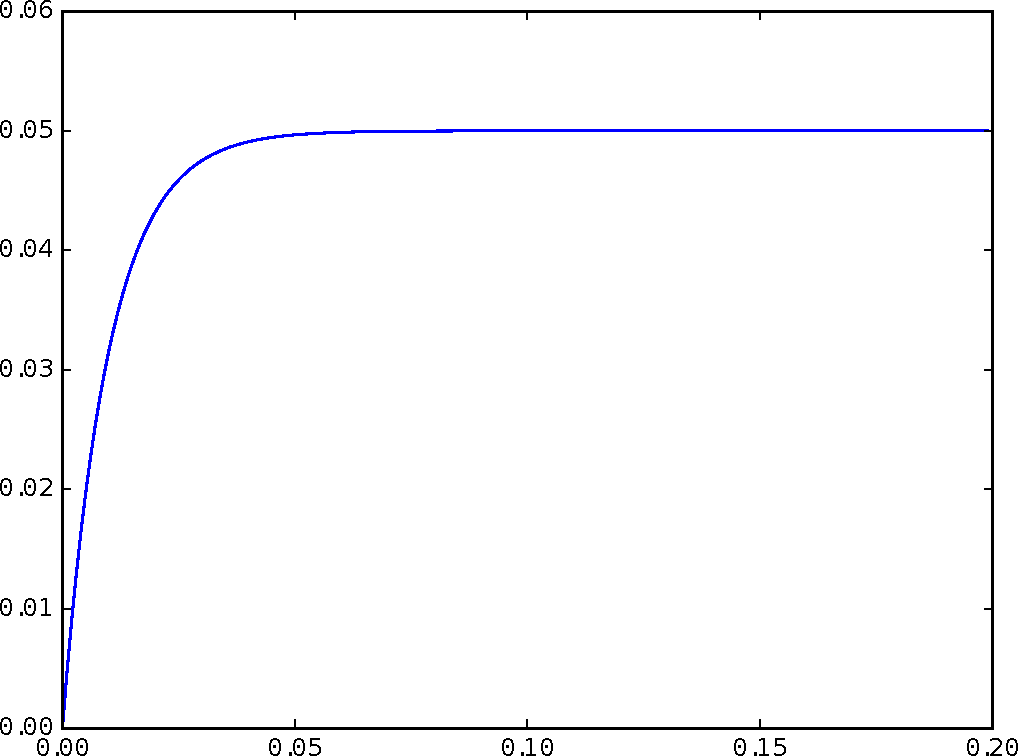
\includegraphics[width=\linewidth]{img/figure_1}
\end{minipage}

\textbf{Question: } Coder la résolution du mouvement oscillatoire d'une masse liée à un ensemble amortisseur/ressort. 

\vspace{3cm}
\end{frame}

\begin{frame}[fragile]
\frametitle{Calcul approché d'équations différentielles}

Il est alors possible de résoudre des systèmes d'équations différentielles.
$\left\{\begin{array}{l} x'(t)=-t*x(t) \\ y'(t)=x(t)+0.2*y(t)
\end{array}\right.$, avec la condition initiale $x(0) = 2$, $y(0) = 1$.

\begin{minipage}{0.6\linewidth}
\begin{GrayBox}[0.92\textwidth]
\begin{verbatimtab}[3]
def f(x, t) :
	f=np.array([-t*x[0], x[0]+0.2*x[1]])
	return f
T = np.arange(0, 5.01, 0.01)
X = integr.odeint(f, np.array([2.,1.]), T)
>>> X
[[  2.00000000e+00   1.00000000e+00]
 [  1.99990000e+00   1.02202166e+00]
 ..., 
\end{verbatimtab}
\end{GrayBox}
\end{minipage}\hfill
\begin{minipage}{0.35\linewidth}
 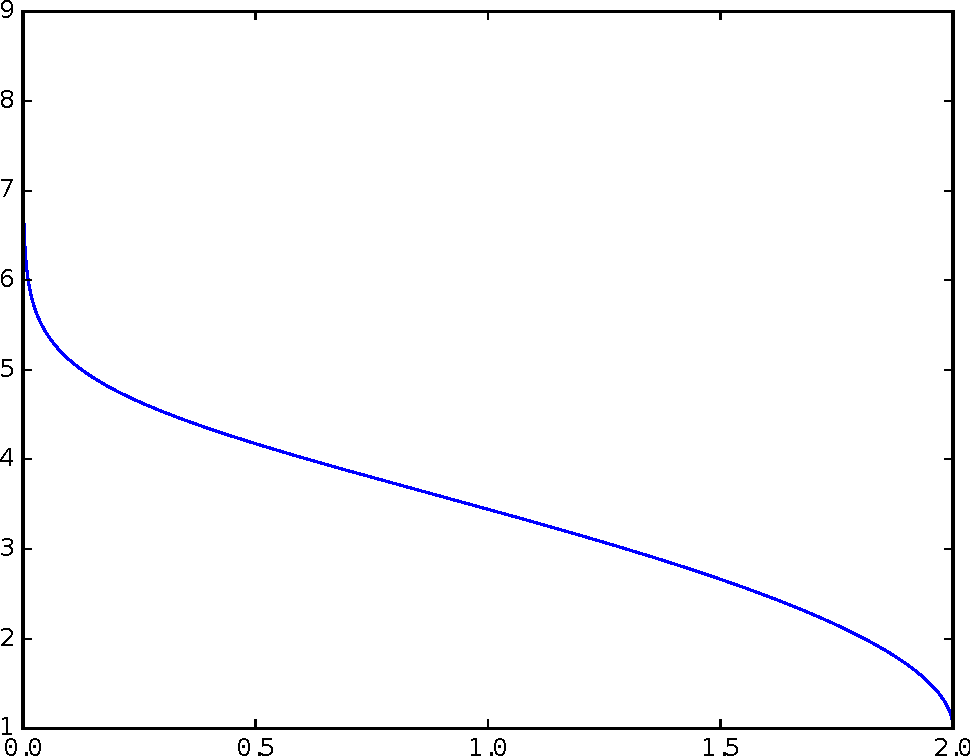
\includegraphics[width=\linewidth]{img/figure_2}
\end{minipage}

Le système d'ordre 1 satisfait par $X(t) = \left(\begin{array}{c}x(t) \\x'(t)\end{array}\right)$ permettra de résoudre une équation différentielle scalaire d'ordre 2 de solution $x$.

\end{frame}

\section{Nombres complexes}

\begin{frame}[fragile]
\frametitle{Nombres complexes}

Avec Python le nombre imaginaire pur $i$ se note \verb? 1j ?. Les attributs \verb? real ? et \verb? imag ? permettent d'obtenir la partie réelle et la partie imaginaire. La fonction \verb? abs ? calcule son module.

\begin{GrayBox}[0.85\textwidth]
\begin{verbatimtab}[3]
>>> a = 6 + 2j
>>> b = 9 - 1j
>>> a*b
(56+12j)
>>> a.real
6.0
>>> a.imag
2.0
>>> abs(a)
6.324555320336759
\end{verbatimtab}
\end{GrayBox}

\end{frame}
\end{document}
